
%%%%%%%%%%%%%%%%%%%%%% Pion, due to Hadron showering %%%%%%%%
\section{Energy loss of particles inside the CMS}
During the collison many particles are produced. Depending on their lifetime, 
they decay to stable particles such electron, photons, etc. The final state 
particles of every collision consist of electron, photon, muon, charged hadrons. 
Based on the kinematic properties of these particles, Other particles such as 
Z/W boson, missing transverse neutrino, jets, Higgs boson, etc are reconstructed.
The various sub-detectors of the CMS are placed in such way so that the occupancy
of a different kind of particles decreases as one goes from tracker to the muon
chambers. The electron and photon is completely stopped in the ECal. The hadrons
($\pi^{\pm}$) deposite their energy partially in the ECal before being completely
stopped in the HCal. Muons are the only particle which reaches to the the muon
chambers. The distacne travelled by various particles and energy loss of these
depend on the type of material used in the calorimeters and the muon chambers.
A brief description of the mechanism of the energy loss of various particles
are given below.

\section{Energy loss of photon and electron}
A photon with energy below few MeV interacts with matter via photoelectric 
effect (emission of electron) and Compton scattering (scattering with charged 
particle). Whereas the photons with high energy, which is case with the photons 
produced in the, the photon interact with material via pair production. A pair
of electron-positron is produced in this process. The electron-positron
subsequntely emit secondary photon by Bremsstrahlung process. These secondary
photon again produce electron-positron pair, as shown in Figure 
(\ref{em_shower}). The pair production and emission continues until the energy
of photon reaches below a certain thresold. Therefore, a shower of particles is
produced in the ECal where energy deposite is spread across various crystal. 
The length of the shower depend on the initial energy of the photon or electron.
\begin{figure}
    \centering
    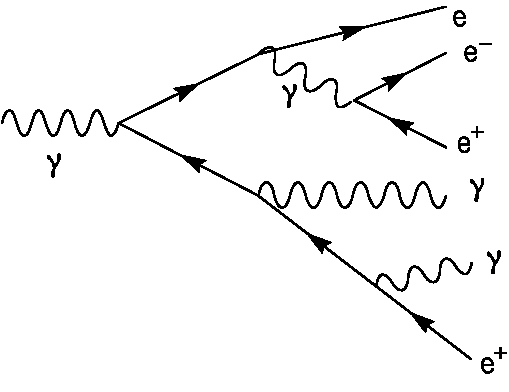
\includegraphics[width=0.50\linewidth]{Experiment/CMS/Image/Loss/em_shower.pdf}
    \caption{Average energy loss of muon in iron vs momentum due to collision. The same plot is shown in Chapter-1, Page-7, Figure-1.1 of the Book[1]}
    \label{fig:em_shower}
\end{figure}

\section{Energy loss of hadrons}
\section{Energy loss of muon}

Charged pion interact with the nuclei through strong forces producing shower of secondary particles.
%\includegraphics[scale=0.5]{hshower.png}
All of the energy of initial hadrons are dumped inside Hcal via this interaction. HS has both EM and Had component.
Energy loss of $\pi^\pm :$ Hadron showering
In-elastic collision is characterised by collision length($\lambda_I$)
\begin{equation}
N = N_0 \exp(-x/\lambda_I), \qquad \lambda_I = \frac{A}{N_A\times \rho\times\sigma_{inel}}
\end{equation}
where $\rho$ is the density, $\sigma_{inel}$ is the total in-elastic cross section of hadrons with the nuclei.
With the initial energy, $E_0$, we can not plot energy loss of charged pion inside Hcal as a function of distance. We can only predict the length of the hadron shower.
The energy deposited due to Hadron showering at the various parts of Hcal is used to reconstruct hadrons.


%%%%%%%%%%%%%%%%%%%%%% Muon, in iron %%%%%%%%
Energy loss of muon in Iron :  Bethe-Bloch
The average energy loss due the collision and ionization is given by Bethe-Bloch formula, Equation 1.11 of [1]

\begin{equation}
-\frac{dE}{dx} =  \frac{\text{K} \left(-\beta ^2+\log \left(\frac{2 \beta ^2 c^2 \gamma ^2
 m_e}{I}\right)-\frac{\delta }{2}\right)}{\beta ^2}
 \label{eq:bethe}
\end{equation}
where
\begin{equation}
K = \frac{4 \pi  c^2 m_e N_A r_e^2 Z}{A}, \quad r_e = \frac{e^2}{4\pi \epsilon_0 m_e c^2}, \quad I = 16Z^{0.9}\times  10^{-3} GeV,
\end{equation}

\begin{equation}
\beta = \left(1-\frac{c^4 m_\mu^2}{m_\mu^2+p^2}\right)^{0.5}, \quad \gamma = \frac{\sqrt{m^2_\mu+p^2}}{c^2 m_\mu}
\end{equation}
and
\begin{equation}
\delta = \log
   \left(2.88\times 10^8
   \sqrt{\frac{\rho  Z}{A}}\right)+2
   \log (\beta  \gamma )-1
\end{equation}

For iron, Z(atomic number) = 26 , A(molar mass) = $55 g/mol$. The constants are given as : $c=3\times10^8 m/s$, $\rho = 7.874g/cm^3, m_e = 9.1\times 10^{-31} Kg, e = 1.6\times 10^{-19}C, N_A = 6.023\times 10^{23}/mol, \frac{1}{4\pi\epsilon_0}= 9\times 10^9 C^2m^{-1}Kg^{-1}s^2$. These constants are in SI unit. Using these, $r_e = 2.813\times 10^{-13} cm$. \\

We want the LHS of Eq.\eqref{eq:bethe} in $MeV/(g/cm^2)$ so to calculate K, $\beta, \gamma, \delta$ we use natural unit convention, keeping $r_e$ in cm. We want to plot a graph between the average energy loss(in $\frac{MeV}{(g/cm^2)}$) and momentum p($GeV/c$).
For this we let c = 1, $m_e = 0.511 MeV, m_\mu = 105.65\times
10^{-3} GeV.$
The plot is shown in the Fig.\ref{fig:muon}.

\begin{figure}
    \centering
    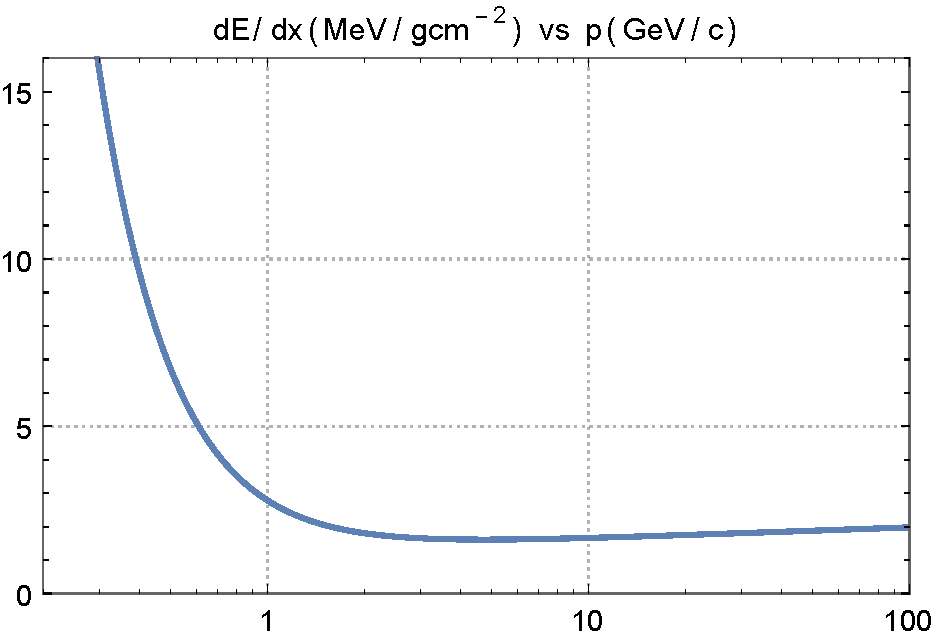
\includegraphics[width=0.50\linewidth]{Experiment/CMS/Image/Loss/muon_iron.pdf}
    \caption{Average energy loss of muon in iron vs momentum due to collision. The same plot is shown in Chapter-1, Page-7, Figure-1.1 of the Book[1]}
    \label{fig:muon}
\end{figure}

Energy loss of charged pion : Bethe-Bloch
Constants for silicon and pion are : $ Z=14, A =28, m_\pi = 0.139 GeV$. The average loss of energy, Eq.\ref{eq:bethe}, of charged pion when they pass through the silicon is plotted against the momentum of muons. The plot is shown Fig.\ref{fig:silicon}.

\begin{figure}
    \centering
    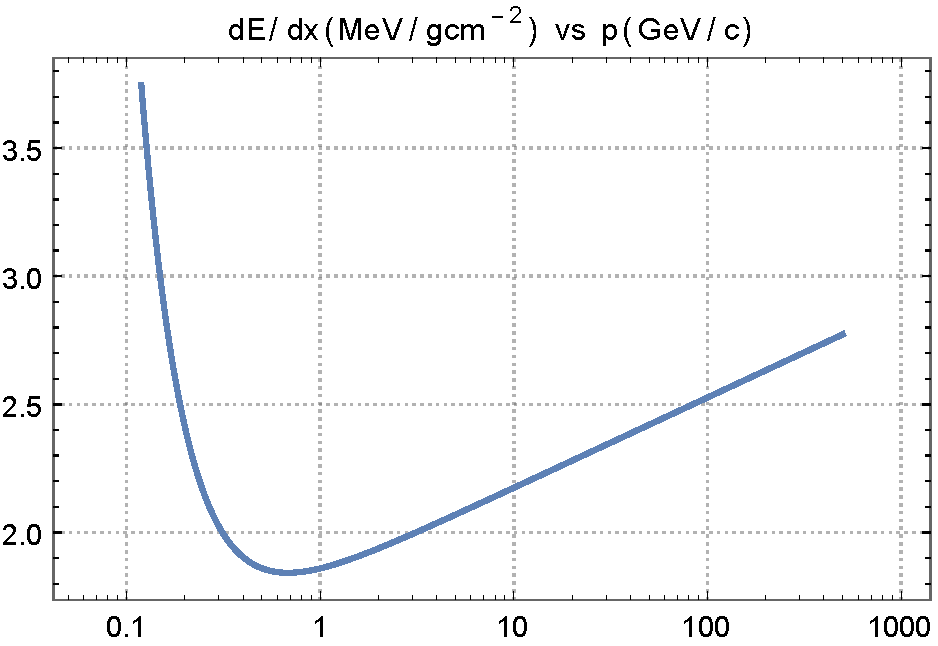
\includegraphics[width=0.50\linewidth]{Experiment/CMS/Image/Loss/pion_silicon_loss.pdf}
    \caption{Average energy loss of pion in silicon vs momentum due to collision}
    \label{fig:silicon}
\end{figure}
Energy loss of charged pion due to collision in silicon tracker
With the initial energy, $E_i^{silicon} = 500 GeV$ the energy loss of charged pion travelling a distance 129cm(radius of silicon tracker) is , $\Delta E^{silicon} = 0.008484 GeV$. So $E_f^{silicon} = 499.992$

Energy loss of charged pion due to collision in EM Calorimeter

The parameters for the Ecal are : Z = 76, A = 455.0376,$\rho =8.3$. The initial energy $E_i^{ecal} = E_f^{silicon} = 499.992$. After travelling a distance 50 cm(295 - 179) the loss is $\Delta E^{ecal} = 0.002969$. So $E^{ecal}_f = 499.902$

Energy loss of charged pion due to collision in Hadron Calorimeter

The parameters for the Hcal are : Z = 29, A = 63.54,$\rho =8.02$. The initial energy $E_i^{hcal} = E_f^{ecal} =  499.902$. After travelling a distance 116 cm(179-129) the loss is $\Delta E^{ecal} = 0.0207$. So $E^{ecal}_f = 499.87$


Energy loss of charge particle due to bremsstrahlung
Energy loss due to bremsstrahlung is given by (x is in $g/cm^2$):
\begin{equation}
-\frac{dE}{dx} = 4\alpha N_A\times \frac{Z^2}{A}\times z^2
\left( \frac{1}{4\pi \epsilon_0}\frac{e^2}{mc^2} \right)^2 \times E\log \frac{183}{Z^{1/3}}
\label{brem}
\end{equation}
\begin{enumerate}
\item Z, A = medium ; E, z, m = incident particle. z =1 for $\pi^\pm$
\item $e = 1.6\times10^{-19} C; c = 3\times10^8 m/s; \alpha = 1/137; N_A = 6.023\times 10^{23}mol^{-1}; m_\pi = 2.48\times 10^{-28} Kg, \frac{1}{4\pi\epsilon_0} = 9\times10^9 Nm^2/C^2 $
\end{enumerate}
Writing Eq\eqref{brem} as $-\frac{dE}{dx} = E/X_0$ we have $E = E_0 \exp(-x/X_0)$
\begin{equation}
\frac{1}{X_0} = 4\alpha N_A\times \frac{Z^2}{A}\times z^2
\left( \frac{1}{4\pi \epsilon_0}\frac{e^2}{mc^2} \right)^2 \times \log \frac{183}{Z^{1/3}}
\end{equation}

\begin{figure}
    \centering
    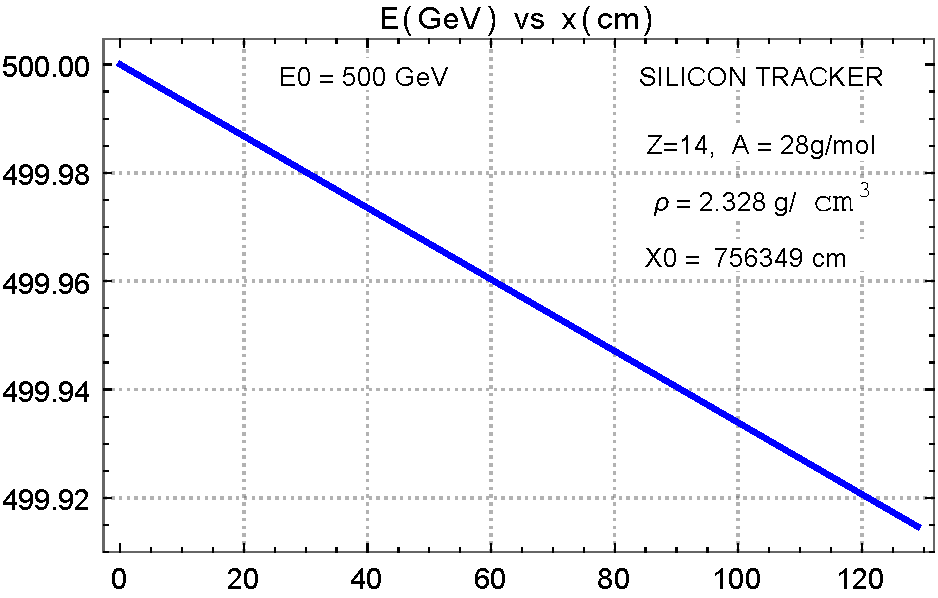
\includegraphics[width=0.50\linewidth]{Experiment/CMS/Image/Loss/pion_silicon.pdf}
    \caption{Energy loss of $\pi^{\pm}$ in silicon detectors due to brem}
    \label{fig:silicon}
\end{figure}

\begin{figure}
    \centering
    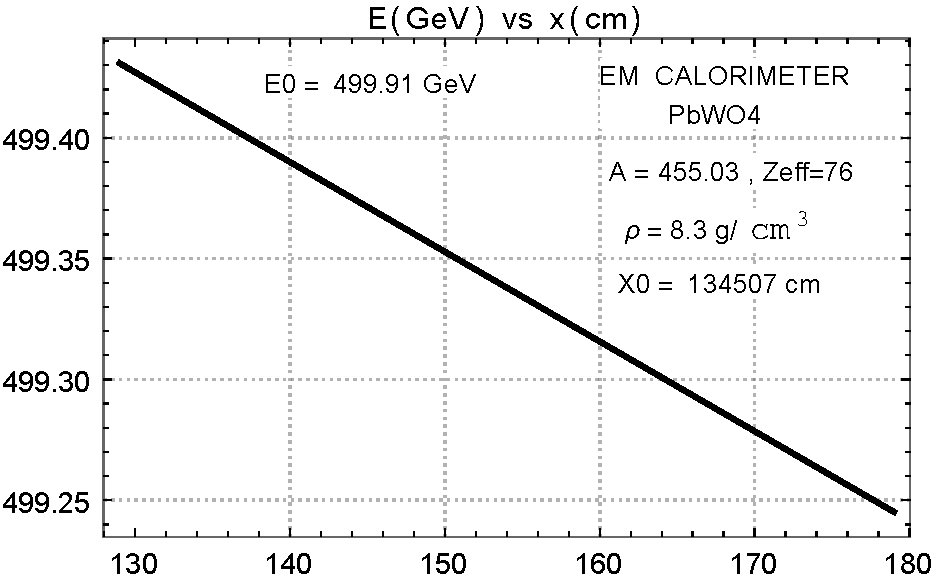
\includegraphics[width=0.50\linewidth]{Experiment/CMS/Image/Loss/pion_ecal.pdf}
    \caption{Energy loss of $\pi^{\pm}$ in EM Cal due to bremsstrahlung}
    \label{fig:silicon}
\end{figure}

\begin{figure}
    \centering
    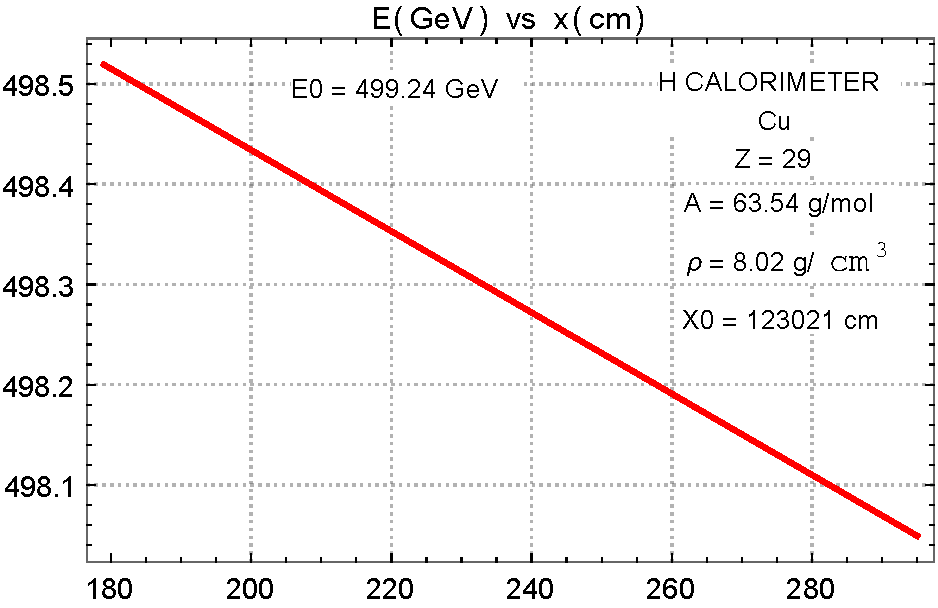
\includegraphics[width=0.50\linewidth]{Experiment/CMS/Image/Loss/pion_hcal.pdf}
    \caption{Energy loss of $\pi^{\pm}$ in HCal due to bremsstrahlung}
    \label{fig:silicon}
\end{figure}

